\documentclass[fleqn,12pt,openany]{book}

% These two need to be set before including scirun style package
\title{SCIRun Developer Guide}
\author{SCIRun Development Team}

% INCLUDE SCI STYLE DOCUMENT
\usepackage{scirun}

\begin{document}

%% starting from SCIRun Doc wiki
%% 


% CREATE TITLE PAGE --------------------------------------------------
\maketitle

\chapter{SCIRun Overview}

SCIRun is a computational workbench used for modeling, simulating and visualizing
scientific problems, which is implemented in C++ with a
Tcl/Tk GUI (Graphical User Interface).
SCIRun uses a dataflow computational model.
SCIRun provides algorithms, math and visualization tools implemented as discrete
software units referred to as \emph{modules}.

Modules are organized into packages: the default package, \emph{SCIRun}, contains general-purpose tools. 
SCIRun can be used on Linux, Mac OS X and Windows platforms.

\chapter{Building SCIRun from Source}

\section{Prerequisites}

\begin{itemize}
\item Subversion
\item CMake (can create XCode projects, GNU make, NMake, Visual Studio)
\item C/C++ compiler
\item GNU make on Linux/Unix platforms
\end{itemize}

The free IDE Visual Studio Express is available for Windows.
Up-to-date prerequisites are available by platform on the \href{http://www.sci.utah.edu/SCIRunDocs/index.php/CIBC:Documentation:SCIRun}{SCIRun documentation wiki}.

\section{Download Sources}

\subsection{Source Archive}

Download the source archive from
\href{http://software.sci.utah.edu}{SCI software portal} from the SCIRun software page.
These are updated regularly, and when a major bug fix has been applied.
Only gzipped tar archives are available at the moment, so Windows users may need to download
thirdparty tools to unpack the archive, such as Cygwin.
The \href{http://www.gzip.org/}{gzip} product page also has a list of tools that can unpack the
archive on Windows.

\subsection{Subversion}

Build SCIRun from the latest sources by checking out code from the
\href{https://code.sci.utah.edu}{SCI Subversion repository}.
We recommend reading \href{http://svnbook.red-bean.com/}{Version Control with Subversion}
for those who have never worked with Subversion before.

%% TODO: repository structure

Usually, the procedure is to check out the code from the
\href{https://code.sci.utah.edu/svn/cibc/cibc/trunk}{repository trunk URL}.

\begin{verbatim}
svn checkout --username anonymous \
  https://code.sci.utah.edu/svn/cibc/cibc/trunk SCIRun
\end{verbatim}

The Installation Guide has detailed information about obtaining SCIRun.

\subsection{Linux and OS X}

Use the CMake tool \textbf{ccmake} to configure the SCIRun build on
the command line.
Make changes to SCIRun's default configuration after configuring
in \textbf{ccmake} for the first time (figure \ref{fig:cmdline-build3}).

\begin{figure}[H]
\scalebox{0.7}{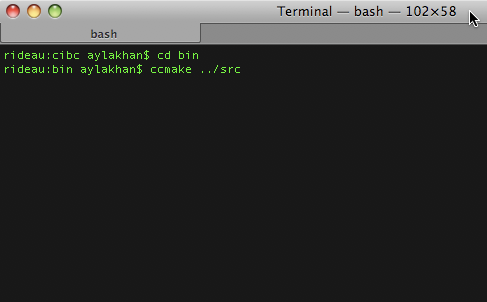
\includegraphics{DeveloperGuide_figures/cmdline_build1.png}}
\caption{CMake tool ccmake on the command line.}
\end{figure}

\begin{figure}[H]
\scalebox{0.6}{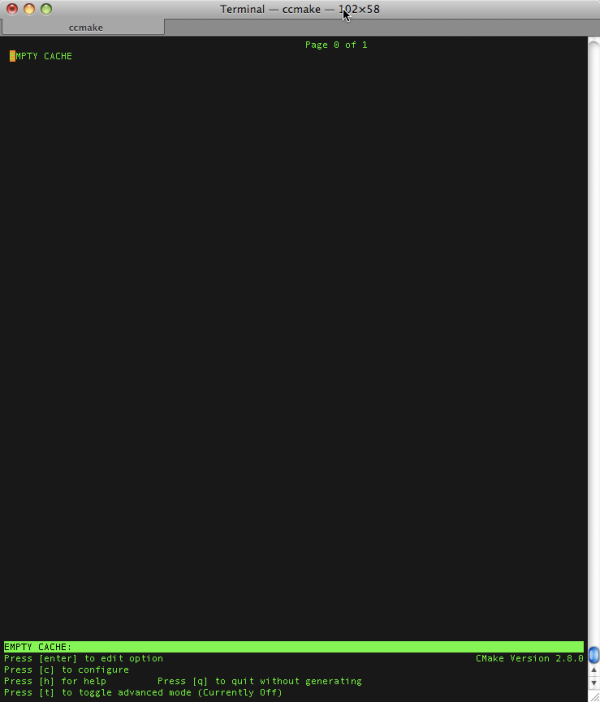
\includegraphics{DeveloperGuide_figures/cmdline_build2.png}}
\caption{CMake tool ccmake interface.}
\end{figure}

\begin{figure}[H]
\scalebox{0.6}{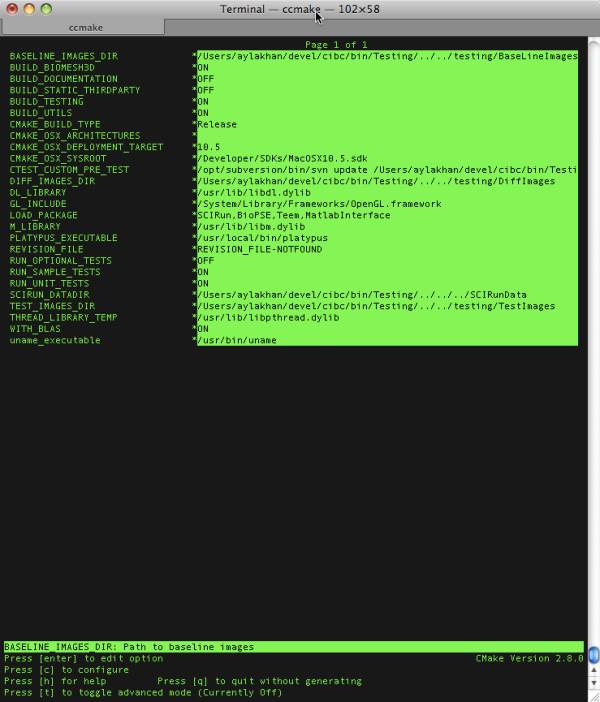
\includegraphics{DeveloperGuide_figures/cmdline_build3.png}}
\caption{CMake tool ccmake interface after configuring for the first time.}
\label{fig:cmdline-build3}
\end{figure}

\begin{figure}[H]
\scalebox{0.7}{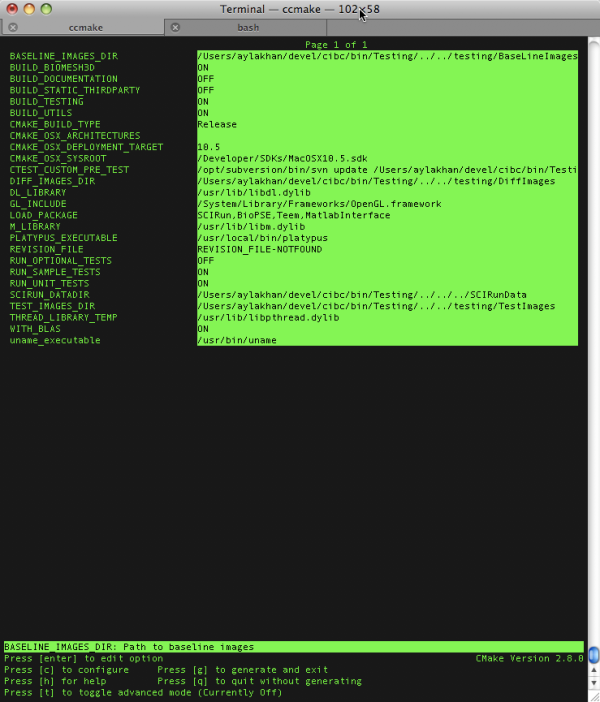
\includegraphics{DeveloperGuide_figures/cmdline_build4.png}}
\caption{CMake tool ccmake interface after configuring for the second time.}
\label{fig:cmdline-build4}
\end{figure}

\begin{figure}[H]
\scalebox{0.7}{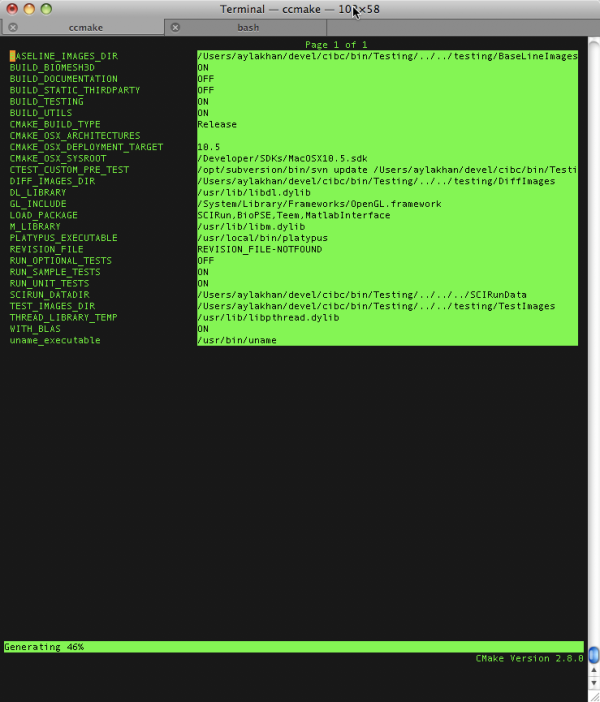
\includegraphics{DeveloperGuide_figures/cmdline_build5.png}}
\caption{CMake tool ccmake interface while generating.}
\end{figure}

%\subsubsection{Troubleshooting CMake builds}

\subsection{Windows}

CMake can generate Visual Studio 2008 project files, which is the only Windows build
solution that we support.
We also recommend using the \textbf{cmake-gui} application.
We suppport both 32 bit and 64 bit builds.

\begin{figure}[H]
\scalebox{0.6}{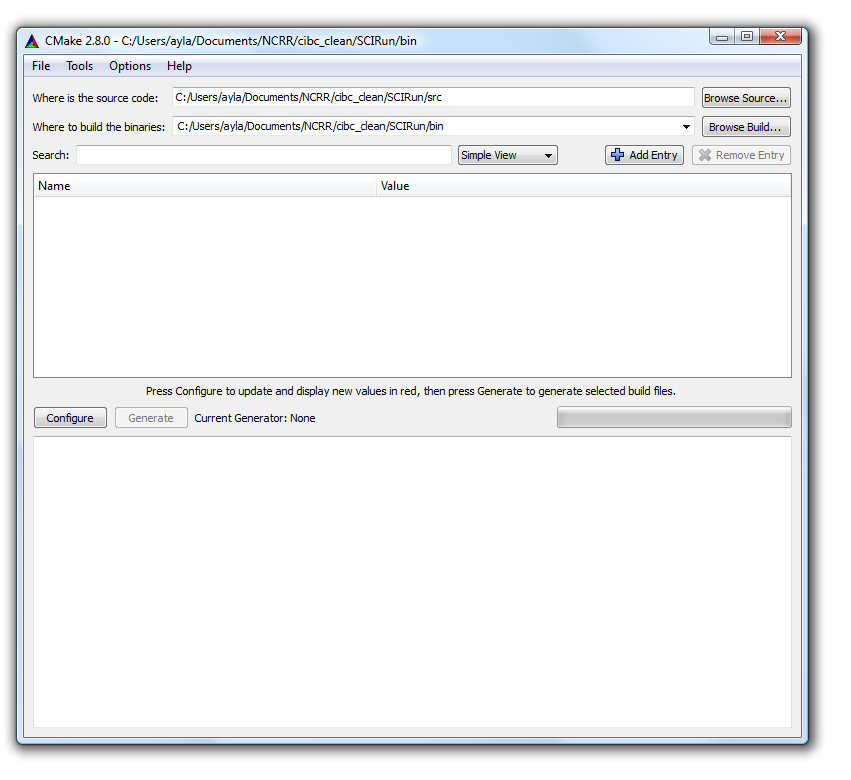
\includegraphics{DeveloperGuide_figures/cmake-gui-windows1.png}}
\caption{CMake GUI with paths to SCIRun source and build directories.}
\label{fig:cmake-gui-windows1}
\end{figure}

\begin{figure}[H]
\scalebox{0.4}{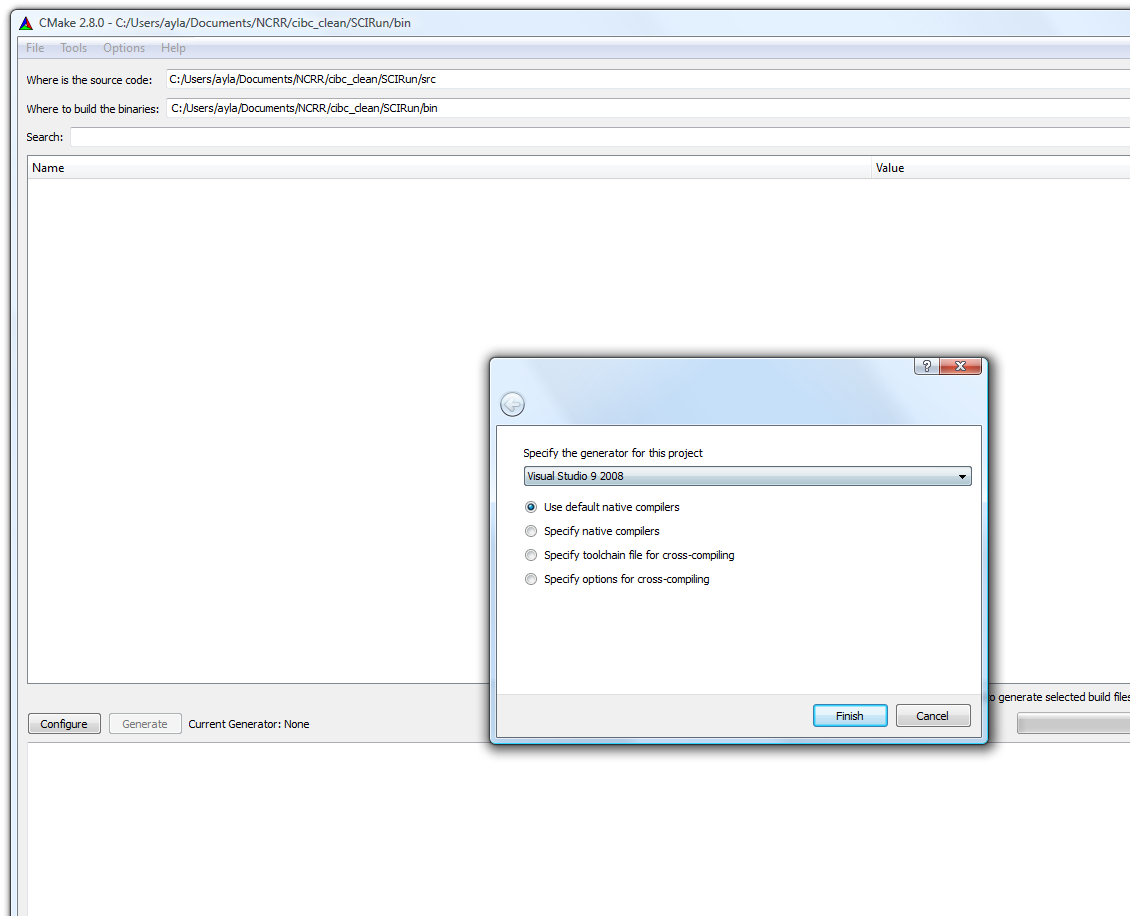
\includegraphics{DeveloperGuide_figures/cmake-gui-windows2.png}}
\caption{CMake GUI select generator for 32 bit Windows build.}
\label{fig:cmake-gui-windows2}
\end{figure}

\begin{figure}[H]
\scalebox{0.4}{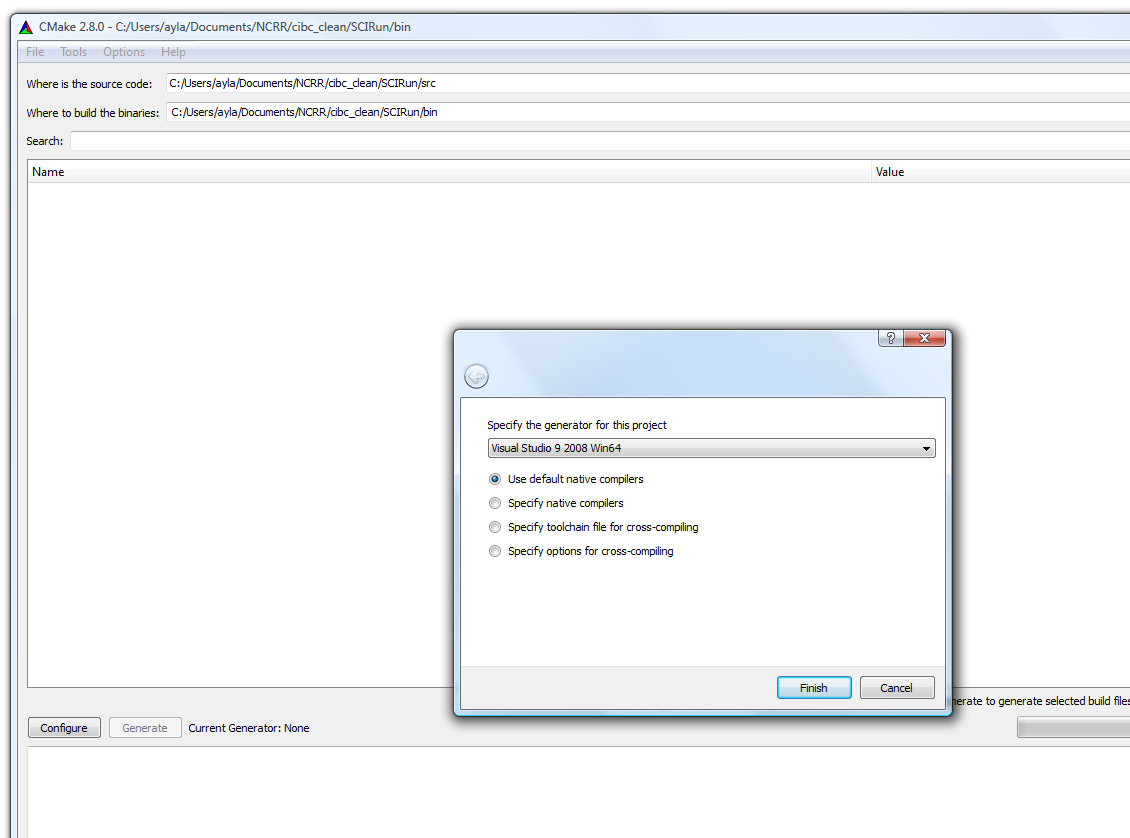
\includegraphics{DeveloperGuide_figures/cmake-gui-windows2_64.png}}
\caption{CMake GUI select generator for 64 bit Windows build.}
\label{fig:cmake-gui-windows2_64}
\end{figure}

\begin{figure}[H]
\scalebox{0.6}{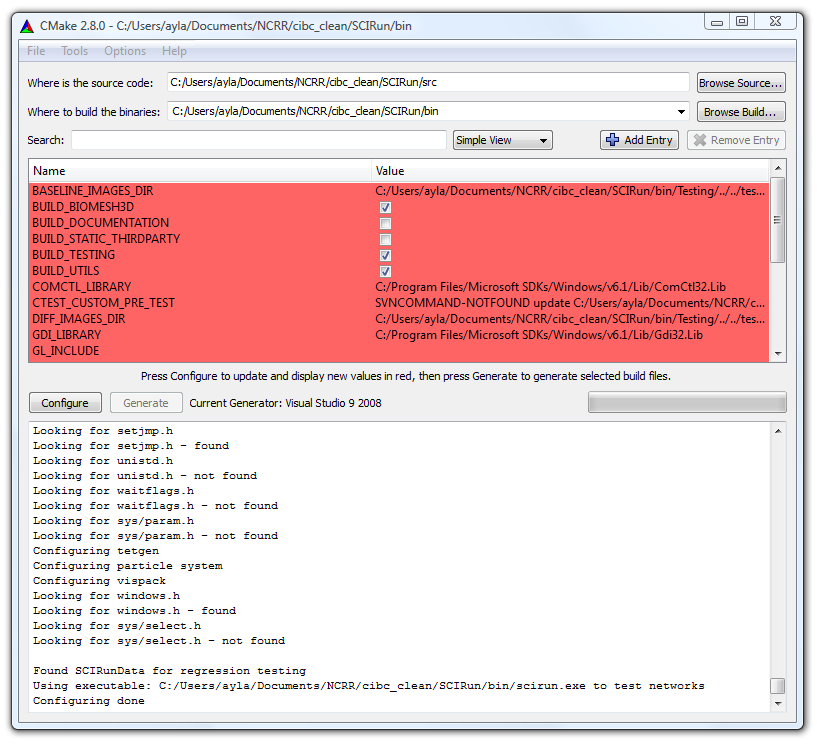
\includegraphics{DeveloperGuide_figures/cmake-gui-windows3.png}}
\caption{CMake GUI after configuring for the first time.}
\end{figure}

\begin{figure}[H]
\scalebox{0.6}{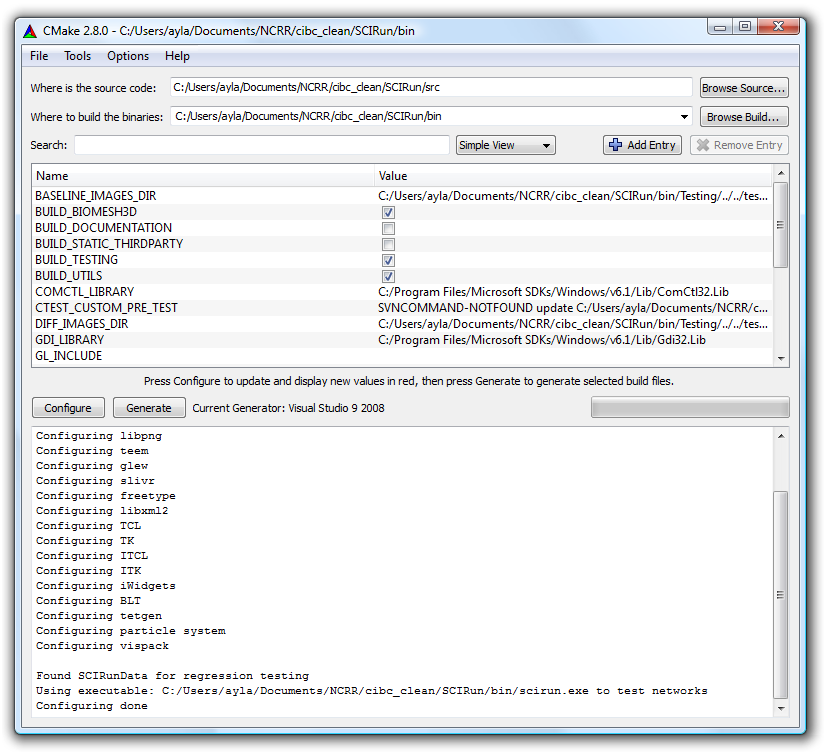
\includegraphics{DeveloperGuide_figures/cmake-gui-windows4.png}}
\caption{CMake GUI after configuring for the second time.}
\end{figure}

\begin{figure}[H]
\scalebox{0.6}{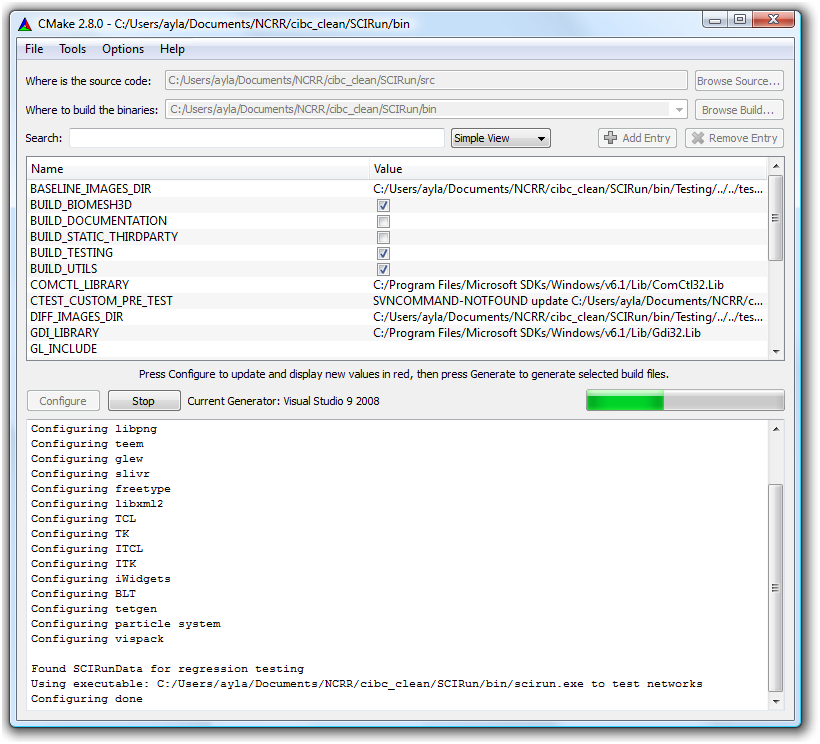
\includegraphics{DeveloperGuide_figures/cmake-gui-windows5.png}}
\caption{CMake GUI while generating.}
\end{figure}

\begin{figure}[H]
\scalebox{0.6}{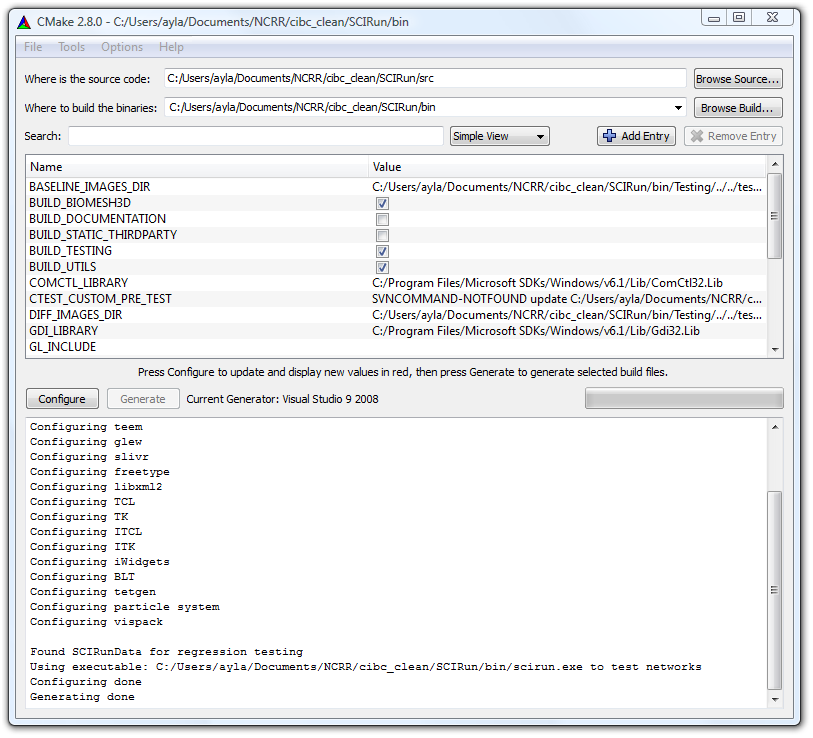
\includegraphics{DeveloperGuide_figures/cmake-gui-windows6.png}}
\caption{CMake GUI after generating.}
\label{fig:cmake-gui-windows6}
\end{figure}

\begin{figure}[H]
\scalebox{0.4}{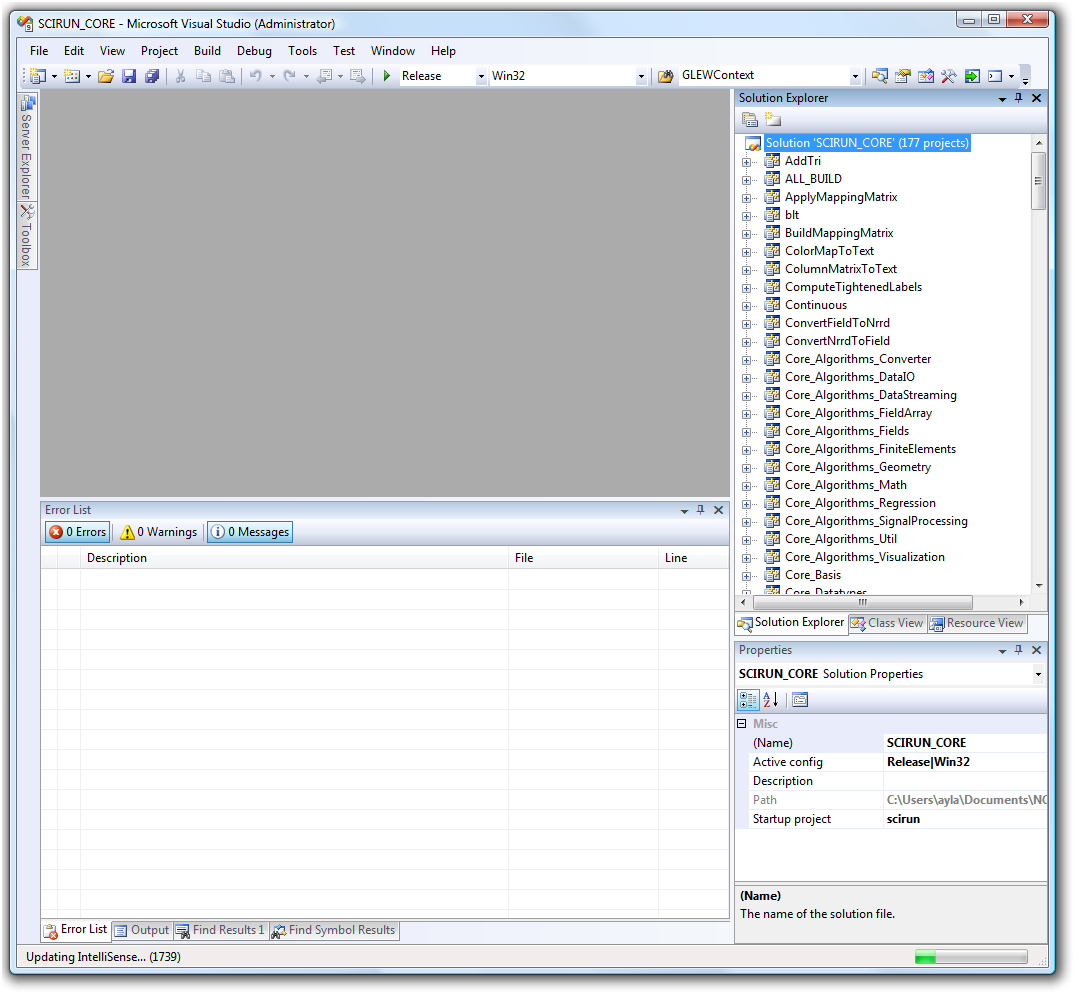
\includegraphics{DeveloperGuide_figures/vs_solution.png}}
\caption{SCIRun Visual Studio solution.}
\label{fig:vs_solution}
\end{figure}

\chapter{Modules}

\section{Tcl Interface}

%% TODO: show an easy Tcl GUI

\section{Communication between Tcl/Tk and C++}

\subsection{GUI Interface}

SCIRun uses Tcl/Tk as its GUI front end.
However, Tcl/Tk was not designed with a clean interface between Tcl code and C/C++.
The purpose of the TCLInterface class in \emph{Dataflow/GuiInterface} is to
provide an abstraction layer make the task of moving data between the Tcl and
the C++ portions of SCIRun transparent to the user.

Most of the code in the \emph{Dataflow/GuiInterface} directory is used internally in SCIRun.
The only exception are the GuiVars which can be access from both the Tcl and the C++ codes.
These variables provide a transparent mechanism in C++ to set or get the Tcl variables
they represent.
Each such Tcl variable is associated with a Module and thus contains information
about the module Tcl ID and a pointer to the module.

\subsection{Programming with the SCIRun GuiInterface}

On the Tcl side, the code should access the variables as regular Tcl variables.
On the C++ side, the code needs to declare these variables inside a Module and
access them via the \texttt{get()} and \texttt{set()} functions.

\subsubsection{GuiVar}

GuiVars are variables that encapsulate the interaction between the C++ code and
the GUI code.
The variable does not hold the actual value, rather it holds information which
is used to access the corresponding variable on the GUI side.
From the C++ side the user may set the variable value using the set() function and
retrieve the value using the get() function.
There are several specialization of the GuiVar class for particular variable types
such as \texttt{GuiInt}, \texttt{GuiString} and \texttt{GuiPoint}.

\noindent In a module's GUI Tcl code:

\begin{verbatim}
 itcl_class foo {
       ...
    method set_defaults {} {
      global $this-min
      global $this-max
      
      set $this-min 0                 # set to 0
      set $this-max [set $this-min]   # '[set $this-var]' returns its value
      }
  ...
 }
\end{verbatim}

\noindent In the C++ side, i.e. in the module class:

\begin{verbatim}
 class Demo : public Module {
    ...
   GuiInt gui_min, gui_max;         // define GUI variables
    
   Demo( const clString& id );
    void init();
 };
  
 Demo::Demo( const clString &id ) 
 : Module(...), 
    gui_min("min",id, this),       // initialize a variable with
    gui_max("max",id,this)         // its name on the Tcl side.
  {
    ...
  }
  
  void Demo::init() 
  {
    gui_min.set(7);               // set a Tcl variable
    int i = gui_max.get();        // get a value from the Tcl side
  }
\end{verbatim}

\chapter{Datatypes}

There are four basic datatypes defined in SCIRun: Field, Matrix, ColorMap, String.
The Nrrd datatype is provided by the Teem package, which wraps the Teem thirdparty project.
The DICOM datatype inteface is provided by Kitware's Insight Toolkit (ITK).

%%\chapter{Algorithms}

%%\chapter{Persistent IO}

\chapter{Import and Exporting File Formats}

SCIRun can read in and write out a variety of file formats through a plugin framework.

\chapter{SCI Coding Standards}

\section{Required Coding Standards}

\begin{itemize}
\item
All code and comments are to be written in English.

\item
All files must include appropriate MIT license information, which must appear at
the top of the file.
Please copy from the LICENSE file at the top of the source tree.
Please update the year to keep the license current.

\item
Include files in C++ always have the file name extension \textbf{.h}.
Use uppercase and lowercase letters in the same way as in the source code.

\item
Implementation files in C++ always have the file name extension \textbf{.cc}.

\item
Every include file must contain a \emph{guard} that prevents multiple
inclusions of the file, for example:

\begin{verbatim}
 #ifndef CORE_GEOMETRY_BBOX_H 
 #define CORE_GEOMETRY_BBOX_H 1
 
 // Code...
 
 #endif
\end{verbatim}

\item
The name of the guard should be of the following form:
\texttt{DIR\_DIR\_FILENAME\_H}

\item
Use forward declarations wherever possible as opposed to including full
definitions for classes, functions, and data:

\begin{verbatim}
 // Class
 class PointToMe;
 
 // Function
 void my_function(PointToMe &p, PointToMe *ptm);
 
 // Data
 PointToMe *m;
\end{verbatim}

Never include /usr/include/*.h, for example iostream.h in any header file.
This causes a huge amount of code to be recursively included an
needlessly compiled.
Use forward declarations to avoid this.

\item
The names of variables and functions will begin with a lowercase letter and
include underscore word separators.
Names of constants should be in all CAPITALS, with underscore word separation:

\begin{verbatim}
 static int CONSTANT_INT_FIVE = 5;
 void my_function_name();
 int my_local_variable_name = 0;
\end{verbatim}

\item
The names of class member variables are to end with an underscore (\texttt{\_}):

\begin{verbatim}
 class MyClass {
   int myClassMember_;
 };
\end{verbatim}

\item
The names of abstract data types (that is, classes), and structs are to begin
with an uppercase letter, and each new word in the name should also be capitalized.

\begin{verbatim}
 class MyNewClassName {
   // ...
 };
\end{verbatim}

\item
All member functions which do not change an object's state should be declared \texttt{const}

\item
Constants are to be defined using \texttt{const} or an enumerated type (\texttt{enum}).
Constant variable names should be all uppercase.
Never use \texttt{\#define} to create constants.

\item
Enumeration member names should be all uppercase and end with \texttt{\_E}.
\begin{verbatim}
    enum my_enum_type {
      // ENUM_CONST_E - some constant I need
      ENUM_CONST_E = 0x0001,
      ...
    };
\end{verbatim}

\item
A class which uses \texttt{new} to allocate instances managed by the class
\textbf{must} define a destructor, a copy constructor and an assignment operator.
If a class needs to define any one of these functions, then all three need to be
present.

\item
Classes should never assume that the input is perfect and a sensible number
of safety checks should be in place to detect faulty inputs. 

\item
Use exception handling to trap errors (although exceptions should only be
used for trapping truly exceptional events).

\item
%% TODO: this should be reviewed at some point...
Our exception model includes two levels of exceptions.
The top level of exceptions are defined in \emph{Core/Exceptions/Exceptions.h}
and are thrown when a class specific exception is not appropriate.
The bottom level of exceptions are class specific, defined in the class that
throws them, and are subclassed off of the top level exceptions.
These class specific exceptions are exceptions that can be caught and handled
from the calling function (1 level above the class).
However, if the calling function chooses not to (or cannot) handle the class
specific exception, the exception will propagate to the next level at which
point it can be trapped and handled in the form of a top level exception.
An example of a class specific exception would be a StackUnderFlowException for a stack class.

\item
Do not use identifiers that begin with an underscore,
such as \texttt{\_myBadIdentifier}.

\item
Do not use \texttt{\#define} to obtain more efficient code; use inline functions instead.

\item
Avoid the use of numeric values (magic numbers) in code; use symbolic values instead.
This applies to numeric values that are repeated within the code but
represent the same value, for example \texttt{MAX\_ARRAY\_SIZE = 1024}.

\item
Do not compare a pointer to \texttt{NULL} or assign \texttt{NULL} to a pointer;
use 0 instead as \texttt{NULL} is not part of the C++ standard and is not
guaranteed to be defined.

\item
Avoid explicit type conversions (casts).
However when a cast is needed, an explicit cast is preferred over having the
compiler decide which kind of cast to do.
Use C++ casts (\texttt{static\_cast}, \texttt{dynamic\_cast} etc.) rather than C-style casts.

\item
Never convert a constant to a non-constant.
Use \texttt{mutable} if necessary, but be aware of the thread safety problems this causes.

\item
\textbf{Never} use \texttt{goto}.
 
\item
Do not use \texttt{malloc}, \texttt{realloc}, or \texttt{free}.
Use \texttt{new} and \texttt{delete} instead.
Allocate arrays on the heap using \texttt{new []} and \texttt{delete []}:

\begin{verbatim}
int *myArray = 0;
myArray = new int[256];
...
delete [] myArray;
\end{verbatim}

%% TODO: public vs. private class members?

\item
Do not use \texttt{long}.
Use \texttt{int} for 32-bit integers and \texttt{long long} for 64-bit integers.

\item
Use C++ STL classes whenever possible instead of writing novel containers.

\item
Do not use C style converters such as \texttt{atoi} because they are not consistently threadsafe on every platform SCIRun supports.
Use the converters in SCIRun's \emph{Core/Util/StringUtil.h} file or STL converters.

\item
Be aware that longs, floats, doubles, long doubles etc. may begin at arbitrary addresses.
Do not assume that built-in data types are contiguous in memory. 

\item
Always use plain \texttt{char} if 8-bit ASCII is used.
Otherwise, use \texttt{signed char} or \texttt{unsigned char}. 

\item
Do not assume that a char is signed or unsigned. 

\item
Do not depend on underflow or overflow functioning in any special way. 

\end{itemize}

\section{Recommended Coding Standards}
\begin{itemize}

\item
Avoid using more than 80 columns per line. 

\item
Group local includes together, then group system includes together. 

\item
Avoid global data if possible. 

\item
Optimize code only if you know that you have a performance problem.
Think twice before you begin. 

\item
When developing new code, always force your compiler to compile with the maximum
warning setting, and before you check in code, fix all warnings. 

\item
Place platform-dependent code in a special file so that it may be easily located
when porting code from one machine to another.
For example, see how platform-dependent thread and synchronization primitive code is organized in \emph{Core/Thread}.

\item
Encapsulate global variables and constants, enumerated types, and typedefs in a class. 

\item
Functions in general should not be more than 30 lines long
(excluding documentation and indentation).
If you find this situation, break the function into several smaller functions.

\item
If a function stores a pointer to an object which is accessed via an argument,
let the argument have the type pointer.
Use reference arguments in other cases. 

\item
When overloading functions, all variations should have the same semantics
(should be used for the same purpose). 

\item
Do not assume that you know how a function's invocation mechanism is implemented. 

\item
Do not assume that an object is initialized in any special order in constructors. 

\item
Use a \texttt{typedef} to simplify program syntax when declaring function pointers
or templated types. 

\item
When two operators are opposites (such as == and !=), it is appropriate to define both. 

\item
Pass function arguments by reference or by constant references (\texttt{const \&})
instead of by value, unless using a built-in data type or a pointer. 

%% TODO: example

\item
Minimize the number of temporary objects that are created as return values from
functions or as arguments to functions. 
Do not write code which is dependent on the lifetime of a temporary object. 

\item
Use C++ streams (i.e. \texttt{std::cout}, \texttt{std::cerr}) instead of \texttt{printf}.
Use C++ streams (i.e. \texttt{std::ostringstream}) instead of \texttt{sprintf}.
Prefer C++ IO streams (i.e. \texttt{std::ifstream}, \texttt{std::ofstream})
to C-style file IO.

\item
Avoid the use of using namespace \texttt{std::} (or other namespaces) in include files,
as they can spill into other files with unintended consequences. 

\item
Try to use smart pointers (\texttt{Handles}) to automatically deallocate memory
when an object is not needed anymore. 

\item
When a function is pure, i.e. it does not modify any of the class members,
annotate it as such so it can be used safely in multi-threaded code. 

\item
When variables are being shared between threads always use a \texttt{Mutex} for access control.
%% TODO: SCIRun supported mutexes
Use a \texttt{Guard} whenever possible to ensure that mutexes are unlocked when
going out of scope.

\item
Use the STL string class and not C-style strings whenever possible. 

\item
Assign a descriptive typename to \texttt{enum} declarations to create a
distinctive type whenever it makes sense to do so.

\begin{verbatim}
  class MyClass {
    ... 
    enum my_enum_type {
      ...
    };
    void my_function(my_enum_type type);
    ...
  };

\end{verbatim}


\end{itemize}

\section{Memory Management}

\subsection{Avoiding Memory Leaks}

%% Proper use of constructors, copy constructors and destructors

%% LockingHandles

Use the SCIRun reference counted LockingHandles wherever possible,
which ensures that memory will be freed when the handle goes out of scope
and the reference count is 0.
The LockingHandle class is defined in \emph{Core/Containers/LockingHandle.h}.
For instance, SCIRun datatypes, if passed as data through a dataflow port
are wrapped in a LockingHandle.

%% TODO: clarifying example

%\section{Thread Management}
%
%SCIRun provides threading, synchronization primitives, and other useful
%classes for managing threads and supporting task parallelism in \emph{Core/Thread}.
%
%Always use the SCIRun thread classes, which wrap platform-specific threading libraries.
%
%% TODO: Thread code example
%
%% TODO: how to use Mutex, Semaphore, Guard etc.

\chapter{Further Reading}

\section{Useful C++ References}

\begin{itemize}
\item
\href{http://www.research.att.com/~bs/3rd.html}{The C++ Programming Language} by Bjarne Stroustrup.
\item
\href{http://mindview.net/Books/TICPP/ThinkingInCPP2e.html}{Thinking in C++} by Bruce Eckel
\item
\href{http://www.aristeia.com/books.html}{Effective C++} by Scott Meyers
\end{itemize}

\end{document}
